\documentclass[11pt,a4paper]{article}

% For å kunne skrive norske tegn.
\usepackage[utf8]{inputenc}

\usepackage{multirow}

% For å inkludere figurer.
\usepackage{graphicx}

% Ekstra matematikkfunksjoner.
\usepackage{amsmath,amssymb}

%\usepackage[section]{placeins}

\usepackage{hyperref}
\hypersetup{%
  colorlinks=true, % hyperlinks will be black
  urlcolor=black,
  linkcolor=black
}

% For å få tilgang til finere linjer (til bruk i tabeller og slikt).
%\usepackage{booktabs}

% For justering av figurtekst og tabelltekst.
%\usepackage[font=small,labelfont=bf]{caption}

% Subsections A, B,
\renewcommand{\thesection}{\arabic{section}}
% \renewcommand{\thesubsection}{\thesection.\arabic{subsection}}

% Disse kommandoene kan gjøre det enklere for LaTeX å plassere figurer og tabeller der du ønsker.
\setcounter{totalnumber}{5}
\renewcommand{\bottomfraction}{0.95}
\renewcommand{\floatpagefraction}{0.35}

\begin{document}

% Rapportens tittel:
\title{Assignment 5: Cluster Validation \\ \large{TDT4300}}
\author{Jonas Myrlund}

% Her ber vi LaTeX om å lage tittelen (til nå har vi bare sagt hva den skal inneholde):
\maketitle

\section{Input file: iris.arff}

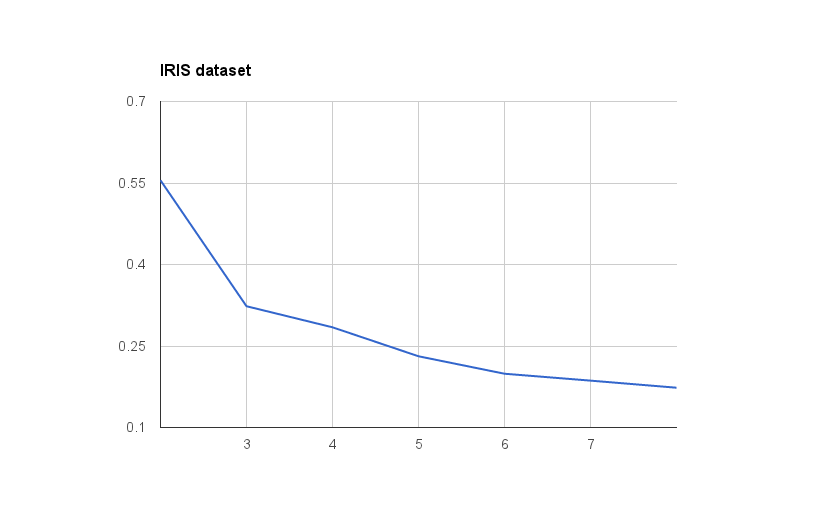
\includegraphics[width=\textwidth]{pics/chart_iris}

\subsection{Results with 2 clusters}
SSE 0.5549309270365081 \\
SSB 6.099212044102275 \\
Sum: 6.654142971138784 \\
Silhouette 0.8230937047026322 \\

\subsection{Results with 3 clusters}
SSE 0.3232076454434727 \\
SSB 6.330935325695304 \\
Sum: 6.654142971138777 \\
Silhouette 0.5874875504843575 \\

\subsection{Results with 4 clusters}
SSE 0.28441408471063384 \\
SSB 6.3697288864281445 \\
Sum: 6.6541429711387785 \\
Silhouette 0.4139987136641223 \\

\subsection{Results with 5 clusters}
SSE 0.2311029082161889 \\
SSB 6.423040062922589 \\
Sum: 6.6541429711387785 \\
Silhouette 0.38433777636479777 \\

\subsection{Results with 6 clusters}
SSE 0.19895796313928532 \\
SSB 6.455185007999494 \\
Sum: 6.654142971138779 \\
Silhouette 0.3518074300182634 \\

\subsection{Results with 7 clusters}
SSE 0.18626798747964463 \\
SSB 6.467874983659131 \\
Sum: 6.654142971138776 \\
Silhouette 0.35026071387060254 \\

\subsection{Results with 8 clusters}
SSE 0.17322281603522888 \\
SSB 6.480920155103546 \\
Sum: 6.654142971138775 \\
Silhouette 0.34073255337201186 \\

\section{Input file: segment-challenge.arff}

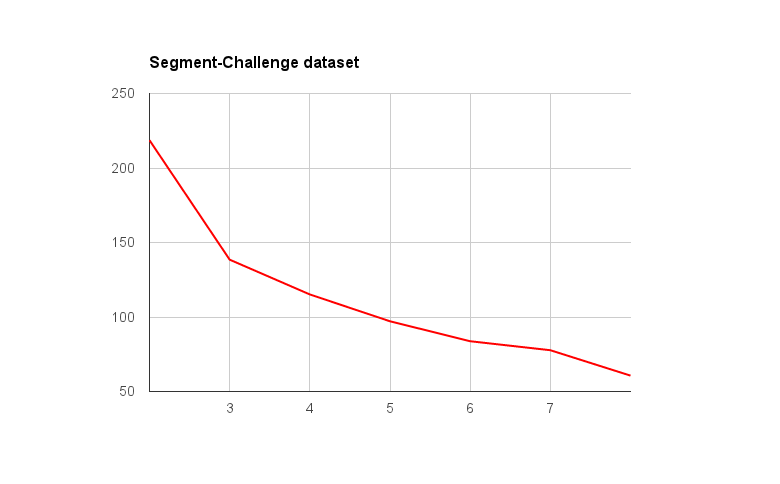
\includegraphics[width=\textwidth]{pics/chart_segment_challenge}

\subsection{Results with 2 clusters}
SSE 218.63399733577185 \\
SSB 146.3036192422363 \\
Sum: 364.93761657800815 \\
Silhouette 0.43376078328594336 \\

\subsection{Results with 3 clusters}
SSE 138.48208000318377 \\
SSB 226.45553657482455 \\
Sum: 364.9376165780083 \\
Silhouette 0.40979463202547517 \\

\subsection{Results with 4 clusters}
SSE 115.13832346281355 \\
SSB 249.79929311519476 \\
Sum: 364.9376165780083 \\
Silhouette 0.37322623437101127 \\

\subsection{Results with 5 clusters}
SSE 97.12357898653049 \\
SSB 267.814037591478 \\
Sum: 364.9376165780085 \\
Silhouette 0.3584521818589955 \\

\subsection{Results with 6 clusters}
SSE 83.73811987818425 \\
SSB 281.1994966998241 \\
Sum: 364.9376165780084 \\
Silhouette 0.37271606896694465 \\

\subsection{Results with 7 clusters}
SSE 77.70794355260699 \\
SSB 287.2296730254016 \\
Sum: 364.9376165780086 \\
Silhouette 0.3600736093766918 \\

\subsection{Results with 8 clusters}
SSE 60.659115522949655 \\
SSB 304.2785010550589 \\
Sum: 364.93761657800854 \\
Silhouette 0.38003837785068945 \\


\end{document}
